\subsection{Funktionsweise}
Wie bereits in Kapitel \ref{lsg:def:anpr} angeführt, besteht die Kennzeichenerkennung aus 3 Schritten. Bevor diese jedoch durchlaufen werden können, müssen zuerst alle notwendigen Bibliotheken installiert und importiert werden. Die meisten können mittels \verb|pip3 install <name>|, oder aber auch mit \verb|sudo apt-get install <name>| installiert werden. \\
Nachdem alle Bibliotheken und das Modul zur Überprüfung des Kennzeichens importiert wurden, beginnt mit \verb|cap = cv2.VideoCapture(0)| das Aufzeichnen des Bildes. Dieses wird durch eine Schleife ausgeführt, bis das Programm beendet wird. Falls die Kamera nicht aufgenommen werden kann, wird eine Fehlermeldung ausgegeben.
\subsubsection{Graustufenbild}
Nachdem das Bild angezeigt wurde, wird der erste Filter angewendet. Dabei handelt es sich um einen Filter, welcher das Bild in ein Graustufenbild umwandelt. Dieser wird  mit der Methode \verb|cv2.cvtColor(img, cv2.COLOR_BGR2GRAY)| aufgerufen.
\begin{figure}[H]
\centering
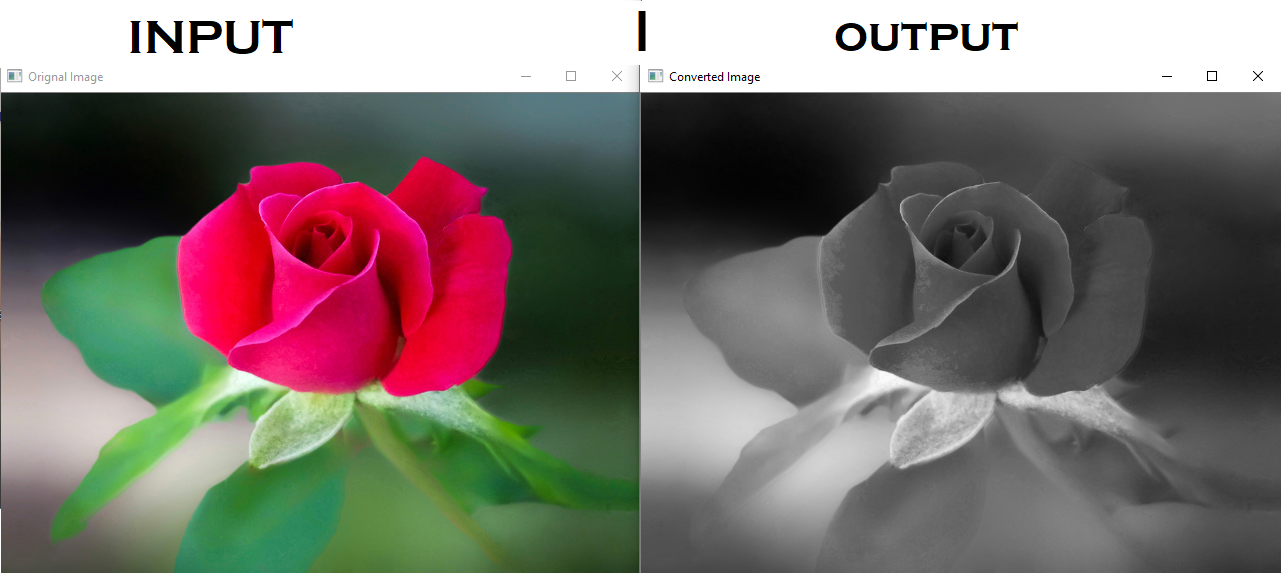
\includegraphics[width=0.8\textwidth]{pics/Color2Gray.PNG}
\caption{Aufgenommenes Bild vs. Graustufenbild}
\cite{grayscaleImage}
\label{fig:anpr_1}
\end{figure}

\subsubsection{Filter}
Als zweiter Filter fungiert ein \verb|cv2.bilateralFilter|. Die wichtigste Eigenschaft der bilateralen Filterung ist, dass sie keine Mittelwertbildung über die Kanten vornimmt. Deshalb wird sie auch als kantenerhaltender Filter bezeichnet.Bevor man sich die mathematischen Grundlagen des Bilateralfilters ansieht, ist es jedoch sinnvoll, kurz auf die Gaußsche Filterung einzugehen, da diese dem bilateralen Filter sehr ähnlich ist.
Die Gaußsche Filterung ist ein gewichteter Durchschnitt der Intensität der benachbarten Positionen, wobei die Gewichtung mit dem räumlichen Abstand zur mittleren Position abnimmt.

Mathematisch gesehen ist ein mit Gaußscher Unschärfe gefiltertes Bild gegeben durch:
\begin{figure}[H]
    \centering
    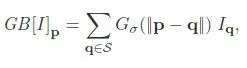
\includegraphics[width=0.5\textwidth]{pics/GBFilteredPic.jpeg}
    \caption{Ein mit Gaußscher Unschärfe gefiltertes Bild}
    \cite{GBfilteredPicture}
    \label{fig:anpr_2}
    \end{figure}
Dabei sind \textit{p} und \textit{q} die Position der Pixel, I kennzeichnet das Bild und G\(\sigma\) (x) den sogenannten zweidimensionalen Gauß-Kernel. 
\begin{figure}[H]
    \centering
    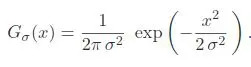
\includegraphics[width=0.5\textwidth]{pics/Gaussian-Filter-Formula-2.jpeg}
    \caption{Gauß-Kernel}
    \cite{GBfilteredPicture2}
    \label{fig:anpr_3}
    \end{figure}
    G\(\sigma\) ist ein räumlicher Gauß, der den Einfluss der entfernten Pixel verringert. Der Abstand zwischen den Pixeln wird mit \(G\sigma(\|p-q\|)\) angegeben. Hierbei ist \(\sigma\) die Ausdehnung der Nachbarschaft.\\
    Der Gaußsche-Unschärfefilter untersucht nur naheliegende Pixel bei der Filterung. Es wird nicht berücksichtig, ob die Pixel die selbe Intensität haben, oder ob die Pixel am Rand liegen oder nicht. Daher werden auch Kanten verwischt, was zu einem Verlust wichtiger Details führt. Die bilaterale Filterung verwendet ebenfalls einen Gauß-Filter im Raum, berücksichtigt aber zusätzlich einen weiteren Gauß-Filter welcher eine Funktion der Pixeldifferenz ist. Die Gaußsche Funktion des Raums sorgt dafür, dass nur nahe gelegene Pixel für die Unschärfe berücksichtigt werden, während die Gaußsche Funktion der Intensitätsdifferenz dafür sorgt, dass nur die Pixel mit ähnlichen Intensitäten wie das zentrale Pixel für die Unschärfe berücksichtigt werden. So bleiben die Kanten erhalten, da die Pixel an den Kanten große Intensitätsunterschiede aufweisen.
    Der wichtige Punkt, der bei der bilateralen Filterung berücksichtigt wird, ist, dass zwei Pixel nicht nur dann nahe beieinander liegen, wenn sie räumlich nahe beieinander liegen, sondern auch, wenn sie eine gewisse Ähnlichkeit im photometrischen Bereich aufweisen. Diese Eigenschaften der bilateralen Filterung überwinden den Nachteil anderer Techniken wie \textit{Averaging Blur} oder \textit{Gaussian Blur}, da sie in der Lage ist, Kanten zu erhalten.\\
    Der Bilaterale Filter wird wie folgt berechnet
\subsubsection{Kantenerkennung}
\cite{Filter}